\section{What happens if $E_{F,e} \neq E_{F,\mu}$?}
\newcommand{\Li}[2]{\mathrm{Li}_{#1}(#2)}
Our starting point is eq. (2.5) of Hong Yi's notes which gives the energy integral under the FSA. It is reproduced here for convenience (taking $n=2$),
\begin{equation}
    J^{(lf)} \equiv \int dE_1 dE_2 dE_1' dE_2' dE_3' ~ {E_3'}^{4} \delta(E_1+E_2-E_1'-E_2'-E_3') f_1 f_2 (1-f_1')(1-f_2') ~.
\end{equation}
The first order of business is to define the variables $x_i \equiv (E_i - {F,i}) / T$ and $z \equiv E_{3}' / T$ and rewrite $J^{(lf)}$ in terms of these variables.
We have,
\begin{equation}
    E_1+E_2-E_1'-E_2'-E_3' = T\,(x_1+x_2-x_1'-x_2'- z) + E_{F,1} + E_{F,2} - E_{F,1}' - E_{F,2}'~.
\end{equation}
However, $2$ is a spectator particle so $E_{F,2} = E_{F,2}'$ ($2$ and $2'$ are the same species of particle). 
Moreover, $E_{F,1} - E_{F,1}'$ is equal to either $T \Delta \equiv E_{F,e} - E_{F,\mu}$ or $- T \Delta = - (E_{F,e} - E_{F,\mu})$ depending on whether ptle 1 is an electron or muon. 
Hence,
\begin{equation}
    E_1+E_2-E_1'-E_2'-E_3' = T\,(x_1+x_2-x_1'-x_2'- z \pm \Delta) ~.
\end{equation}
\begin{equation}
    J^{(lf)}(\Delta) = \int T^5 \,\dd x_1 \dd x_2 \dd x_1' \dd x_2' \dd z ~ T^4 {z}^{4} 
    \frac{\delta(x_1 + x_2 - x_1' - x_2' - z \pm \Delta)}{T}  f_1 f_2 (1-f_1')(1-f_2') ~,
\end{equation}
where the upper sign $(+)$ is for $l = e$ and the lower sign $(-)$ is for $l = \mu$.
This simplifies to a modified form of Hong Yi's eq. (2.8) when we assume strongly degenerate particles (so that the integrals over $x_i$ are from $-\infty$ to $+\infty$).
\begin{equation}
    \label{eq:hong-yi-2.8}
    J^{(lf)}(\Delta) = 
    \int_{-\infty}^\infty \! \dd x_1
     \dd x_2
     \dd x_1'
     \dd x_2'
    \int_0^\infty \dd z
    \frac{
        T^{8} z^{4} \, \delta(x_1 + x_2 - x_1' - x_2' - z  \pm \Delta)
    }
    {
        (e^{x_1} + 1)
        (e^{x_2} + 1)
        (e^{-x_1'} + 1)
        (e^{-x_2'} + 1)
    } ~.
\end{equation}
The $x_i$ integrals in \eref{eq:hong-yi-2.8} can be evaluated by doing the change of variables $\tilde{z} = z \mp \Delta$ and using the formula,
\begin{equation*}
\begin{aligned}
    \int_{-\infty}^{\infty} \! \dd x_1 \cdots \dd x_4 \, 
    \frac{
        \delta(x_1 + x_2 + x_3 + x_4 - \tilde{z})
    }{
        (e^{x_1} + 1)
        (e^{x_2} + 1)
        (e^{x_3} + 1)
        (e^{x_4} + 1)
    }
    = 
    \frac{1}{6} \frac{\tilde{z} \, (\tilde{z}^2 + 4\pi^2)}{e^{\tilde{z}} - 1}~,
\end{aligned}
\end{equation*}
so that we obtain
\begin{equation}
    \label{eq:J-only-z-integral}
    J^{(lf)}(\Delta) = 
    \frac{T^8}{6}
    \int_\Delta^\infty \! \dd \tilde{z} \  (\tilde{z} \pm \Delta)^4 \, 
    \frac{\tilde{z} \, (\tilde{z}^2 + 4\pi^2)}
    {e^{\tilde{z}} - 1}~.
\end{equation}
\Eref{eq:J-only-z-integral} can be evaluated analytically for any $\Delta$ but in the special case $\Delta = 0$ the result is $J^{(lf)} (0) = (164 \, \pi^8 / 945) \, T^8$, and is independent of the process.
We now consider the cases $J^{(ef)}$ and $J^{(\mu f)}$.

\underline{$ef \rightarrow \mu f a$:} \vspace{1ex} \newline 
In this case, we evaluate \eref{eq:J-only-z-integral} with the upper sign $(+)$.
Mathematica can do this analytically and we obtain
\begin{equation}
\begin{aligned}
    \label{eq:J-positive-delta}
    J^{(ep)}(\Delta) &= 
    \frac{T^{8}}{6} \int_\Delta^\infty \! \dd \tilde{z} \  (\tilde{z} + \Delta)^{4} \, \frac{\tilde{z} \, (\tilde{z}^2 + 4\pi^2)}{e^{\tilde{z}} - 1} \\
    &= 
    4 \, [
        210 \, \Li{8}{e^\Delta}
        - 90 \, \Delta \, \Li{7}{e^\Delta}
        + 5 \, (4\pi^2 + 3 \Delta^2) \, \Li{6}{e^\Delta}
        - (4\pi^2 \, \Delta + \Delta^3) \, \Li{5}{e^\Delta}
    ]
    ~,
\end{aligned}
\end{equation}
where $\Li{n}{x}$ is the polylogarithm function (see \texttt{PolyLog} in Mathematica's documentation).
As expected, this coincides with $(164 \, \pi^8 / 945) \, T^8$ when $\Delta = 0$.
As shown in \fref{fig:positive-delta} \eqref{eq:J-positive-delta} is well approximated by an exponential decay of the form $e^{-k \Delta}$.  
\begin{figure}[htbp]
    \centering
    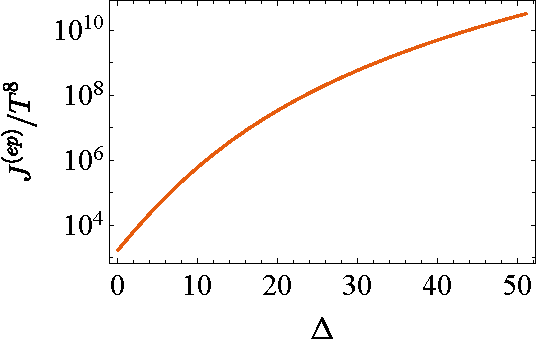
\includegraphics[width=0.45\linewidth]{figs/polylogarithm.pdf}
    \includegraphics[width=0.45\linewidth]{figs/epdata.pdf}
    \caption{
        \emph{Left}:
        Plotting the polylogarithm function given in \eref{eq:J-positive-delta} versus $\Delta$.
        At $\Delta=0$ this coincides with $(164 \, \pi^8 / 945) \, T^8 \approx 1650 \, T^8$. For $\Delta < 10$ this is well-approximated by an exponential enhancement.
        \emph{Right}: 
        Numerically evaluated emissivity versus $\Delta$.
        Notice that the behaviour is the same. This gives me confidence that the discussion here is a sufficient explanation.
    }
    \label{fig:positive-delta}
\end{figure}

\underline{$\mu f \rightarrow e f a$:} \vspace{1ex} \newline
In this case, we evaluate \eref{eq:J-only-z-integral} with the lower sign $(-)$.
Mathematica can do this analytically and we obtain
\begin{equation}
\begin{aligned}
    \label{eq:J-positive-delta-up}
    \frac{J^{(\mu f)}(\Delta)}{T^8} = 
    4 \, T^8 \big[
        (4 \pi^2 \Delta + \Delta^3) \, \Li{5}{e^{-\Delta}}
        + 5 (4\pi^2 + 3 \Delta^2) \, \Li{6}{e^{-\Delta}}
        + 90 \Delta \, \Li{7}{e^{-\Delta}}
        + 210 \, \Li{8}{e^{-\Delta}}
    \big]~,
\end{aligned}
\end{equation}

\begin{figure}[htbp]
    \centering
    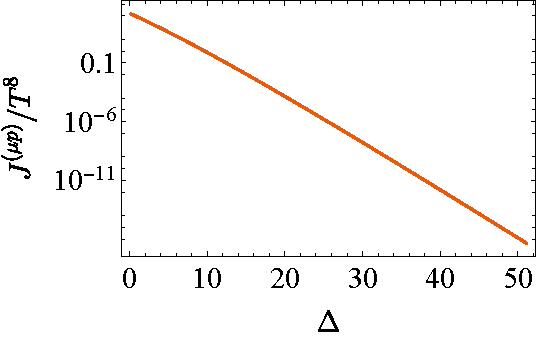
\includegraphics[width=0.45\linewidth]{figs/polylogarithm-2.pdf}
    \includegraphics[width=0.45\linewidth]{figs/updata.pdf}
    \caption{
        \emph{Left}: The polylogarithm function given in \eref{eq:J-positive-delta-up} versus $\Delta$. At $\Delta=0$ this coincides with $(164 \, \pi^8 / 945) \, T^8 \approx 1650 \, T^8$. This is well-approximated by an exponential decay.
        \emph{Right}: Numerically evaluated emissivity versus $\Delta$.
        Notice that the behaviour is the same. This gives me confidence that the discussion here is a sufficient explanation.
    }
    \label{fig:positive-delta-up}
\end{figure}

